\DocumentMetadata{
    lang=pt-BR,
    pdfstandard=ua-2,
    testphase={phase-III,math,table,title,graphic}
}

\documentclass[12pt,a4paper]{article}

% =========================================
% FONTE ARIAL (XeLaTeX)
% =========================================

\usepackage{fontspec}
\setmainfont{Arial}

% =========================================
% IDIOMA
% =========================================

\usepackage[brazil]{babel}

% =========================================
% LAYOUT DA PÁGINA
% =========================================

\usepackage[
    a4paper,
    top=96pt,
    bottom=96pt,
    left=96pt,
    right=96pt
]{geometry}


% =========================================
% PACOTES GERAIS
% =========================================

\usepackage{graphicx}
\usepackage{hyperref}

% Legendas (figuras e tabelas)
\usepackage{caption}

\DeclareCaptionFont{legendafont}{
    \fontsize{10pt}{12pt}\selectfont
}

\captionsetup{
    font=legendafont
}

\usepackage{enumitem}

\usepackage{float}
\usepackage[section]{placeins} % impede figuras/tabelas de irem muito longe (não ultrapassam a seção)
\usepackage{array}
\usepackage[table]{xcolor} % cores em tabelas (cronograma)
\usepackage{longtable}
\usepackage{booktabs}
\usepackage{multirow}
\usepackage[alf]{abntex2cite}
\usepackage{tabularx}

% =========================================
% CÁLCULOS E AUTOMATIZAÇÃO (FÓRMULA GERAL)
% =========================================
\usepackage{xfp}
\usepackage{siunitx}
\sisetup{output-decimal-marker = {,}}

% Comando: \media{soma}{quantidade}
\newcommand{\media}[2]{%
    \num{\fpeval{round((#1)/(#2), 1)}}%
}
% =========================================
% ESPAÇAMENTO E ALINHAMENTO
% =========================================
\usepackage{ragged2e}
\AtBeginDocument{%
    \setlength{\parindent}{0pt}%
    \setlength{\parskip}{15pt}%
}

\hyphenpenalty=10000
\exhyphenpenalty=10000
\sloppy

\frenchspacing

% =========================================
% ESTILO DAS SEÇÕES
% =========================================

\usepackage{titlesec}

\titleformat{\section}
{\normalfont\fontsize{14pt}{14pt}\bfseries\raggedright}
{\thesection.}
{1.5em}
{}

\titleformat{\subsection}
{\normalfont\fontsize{12pt}{12pt}\bfseries\itshape\raggedright}
{\thesubsection}
{0.2em}
{}

\titleformat{\subsubsection}
{\normalfont\normalsize\raggedright}
{\thesubsubsection}
{0.2em}
{}

% =========================================
% ESPAÇAMENTO DOS TÍTULOS
% =========================================

\titlespacing*{\section}
{0pt}
{0pt}
{-14pt}

\titlespacing*{\subsection}
{4pt}
{4pt}
{-15pt} 

\titlespacing*{\subsubsection}
{4pt}
{4pt}
{-15pt}

% =========================================
% LINKS
% =========================================

\hypersetup{
    colorlinks=false,
    linkcolor=black,   % Cor dos links internos (sumário)
    urlcolor=black,    % Cor de links externos (sites)
    citecolor=black    % Cor das citações no texto (Isto remove o colorido das citações)
}

% =========================================
% LOGO FIXO EM TODAS AS PÁGINAS
% =========================================

\usepackage{eso-pic}

\AddToShipoutPictureBG{
    \put(480,740){
        
\includegraphics[
            width=3.3cm,
            alt={Logo CESAR School}
        ]{images/cesar_school_logo.png}
    }
}

% =========================================
% REMOVE NUMERAÇÃO DAS PÁGINAS
% =========================================

\pagestyle{empty}
\setlength{\parindent}{1.25cm}
\setlength{\parskip}{0.2cm}

\hypersetup{
    colorlinks=true,
    linkcolor=blue,
    urlcolor=blue,
    citecolor=blue
}

\bibliographystyle{abntex2-alf}

\begin{document}
% =========================================
% CAPA
% =========================================

\begin{titlepage}

\begin{center}

{\large \textbf{CENTRO DE ESTUDOS E SISTEMAS AVANÇADOS DO RECIFE}}\\[0.5cm]

{\large GRADUAÇÃO EM CIÊNCIA DA COMPUTAÇÃO}

\vspace{7cm}

{\Large \textbf{<TÍTULO DO PROJETO DE PESQUISA>}}

\vspace{7cm}

<NOME DOS ALUNOS>\\[0.2cm]
<NOME DO ORIENTADOR>\\[0.2cm]
<NOME DO CO-ORIENTADOR -- opcional>

\vspace{1.5cm}

Recife, <mês> de 2026.

\end{center}

\end{titlepage}


% =========================================
% INTRODUÇÃO
% =========================================

\newpage
\section{Introdução}

\vspace{-0.4cm}

\noindent\rule{\textwidth}{0.7pt}

Descreva aqui uma breve apresentação do capítulo 1.

\subsection{Motivação e Contexto}

<Análise e delimitação da situação inicial do problema de pesquisa. Aborde os assuntos relacionados ao tema que serão estudados. Detalhe as motivações por exemplo [científicas, técnicas, mercado, etc] relatando quais inovações e/ou pesquisas estão motivando o desenvolvimento do trabalho. Aqui você precisa despertar o interesse do leitor em sua pesquisa.>

\textcolor{red}{
<Os parágrafos produzidos precisam fazer uso de citações.
O recomendável é 1 citação (direta ou indireta)
para cada 2 parágrafos produzidos.>
}

\subsection{Problema de Pesquisa}

<Descreva com detalhes o seu problema de pesquisa.  <[Lembre-se do que foi conversado em sala de aula, sobre os elementos que compõem a problematização].>


\textcolor{red}{
<Os parágrafos produzidos precisam fazer uso de citações.
O recomendável é 1 citação (direta ou indireta)
para cada 2 parágrafos produzidos.>
}

<E por fim, resuma a problemática em uma pergunta
que irá nortear sua pesquisa.>

\subsection{Justificativa}

Descrever a justificativa para realização da pesquisa, explicando por que o problema é relevante. Aqui você precisa deixar clara a importância da sua pesquisa. Cite as vantagens que sua pesquisa irá trazer em relação ao problema de pesquisa.

\textcolor{red}{
<Os parágrafos produzidos precisam fazer uso de citações.
O recomendável é 1 citação (direta ou indireta)
para cada 2 parágrafos produzidos.> 
}

\subsection{Objetivos}
<Escrever, ao menos, um parágrafo introdutório para a seção de objetivos da pesquisa.>

\subsubsection{Objetivo Geral}

<Definição do objetivo geral.>

\subsubsection{Objetivos Específicos}

\vspace{0.7cm}

\begin{itemize}[label=$\bullet$]
    \item OE 1
    \item OE 2
    \item OE 3
    \item OE N
\end{itemize}

% =========================================
% SOLUÇÕES EXISTENTES
% =========================================

\newpage
\section{Soluções Existentes}

\vspace{-0.4cm}

\noindent\rule{\textwidth}{0.7pt}

<Se optar pelo capítulo de Soluções Existentes: Identificar e descrever soluções existentes para o problema de pesquisa definido. Detalhar como estas soluções atendem o problema, em que aspectos ou necessidades elas atendem. E descrever em que as soluções existentes deixam a desejar, ou seja, no que não atendem ao problema. Ao final realizar uma análise comparativa entre as soluções existentes. Mínimo de 5 soluções>

<É obrigatório organizar as soluções existentes em uma estrutura de tópicos.>

\subsection{Solução Existente 1}

<Em um texto corrido, faça a apresentação detalhada da solução. Explique o objetivo da solução, como usar, a aplicabilidade, histórico de sucesso, quando foi criado, quem criou, e o que mais julgar se necessário para explicar a solução.>

\textcolor{red}{
<Os parágrafos produzidos precisam fazer uso de citações.
O recomendável é 1 citação (direta ou indireta)
para cada 2 parágrafos produzidos.>
}

\subsubsection{Aspectos Positivos de Atendimento ao Problema}
<Texto do Tópico> É para detalhar e explicar cada aspecto e não somente citar eles.

\subsubsection{Aspectos Negativos de Atendimento ao Problema}
<Texto do Tópico> É para detalhar e explicar cada aspecto e não somente citar eles.

\subsection{Solução Existente 2}

<Em um texto corrido, faça a apresentação detalhada da solução. Explique o objetivo da solução, como usar, a aplicabilidade, histórico de sucesso, quando foi criado, quem criou, e o que mais julgar se necessário para explicar a solução.>

\textcolor{red}{
<Os parágrafos produzidos precisam fazer uso de citações.
O recomendável é 1 citação (direta ou indireta)
para cada 2 parágrafos produzidos.>
}

\subsubsection{Aspectos Positivos de Atendimento ao Problema}
<Texto do Tópico> É para detalhar e explicar cada aspecto e não somente citar eles.

\subsubsection{Aspectos Negativos de Atendimento ao Problema}
<Texto do Tópico> É para detalhar e explicar cada aspecto e não somente citar eles.

\subsection{Solução Existente 3}

<Em um texto corrido, faça a apresentação detalhada da solução. Explique o objetivo da solução, como usar, a aplicabilidade, histórico de sucesso, quando foi criado, quem criou, e o que mais julgar se necessário para explicar a solução.>

\textcolor{red}{
<Os parágrafos produzidos precisam fazer uso de citações.
O recomendável é 1 citação (direta ou indireta)
para cada 2 parágrafos produzidos.>
}

\subsubsection{Aspectos Positivos de Atendimento ao Problema}
<Texto do Tópico> É para detalhar e explicar cada aspecto e não somente citar eles.

\subsubsection{Aspectos Negativos de Atendimento ao Problema}
<Texto do Tópico> É para detalhar e explicar cada aspecto e não somente citar eles.

\subsection{Solução Existente 4}

<Em um texto corrido, faça a apresentação detalhada da solução. Explique o objetivo da solução, como usar, a aplicabilidade, histórico de sucesso, quando foi criado, quem criou, e o que mais julgar se necessário para explicar a solução.>

\textcolor{red}{
<Os parágrafos produzidos precisam fazer uso de citações.
O recomendável é 1 citação (direta ou indireta)
para cada 2 parágrafos produzidos.>
}

\subsubsection{Aspectos Positivos de Atendimento ao Problema}
<Texto do Tópico> É para detalhar e explicar cada aspecto e não somente citar eles.

\subsubsection{Aspectos Negativos de Atendimento ao Problema}
<Texto do Tópico> É para detalhar e explicar cada aspecto e não somente citar eles.

\subsection{Solução Existente 5}

<Em um texto corrido, faça a apresentação detalhada da solução. Explique o objetivo da solução, como usar, a aplicabilidade, histórico de sucesso, quando foi criado, quem criou, e o que mais julgar se necessário para explicar a solução.>

\textcolor{red}{
<Os parágrafos produzidos precisam fazer uso de citações.
O recomendável é 1 citação (direta ou indireta)
para cada 2 parágrafos produzidos.>
}

\subsubsection{Aspectos Positivos de Atendimento ao Problema}
<Texto do Tópico> É para detalhar e explicar cada aspecto e não somente citar eles.

\subsubsection{Aspectos Negativos de Atendimento ao Problema}
<Texto do Tópico> É para detalhar e explicar cada aspecto e não somente citar eles.

\subsection{ Análise Comparativa das Soluções Existentes}
<Analise as 5 soluções existentes comparativamente sob a óticas dos critérios pertinentes aos problemas de pesquisa. Para isto, crie uma tabela para apresentar os pontos em comum e divergentes entre as soluções selecionadas.>


\begin{table}[htbp]
\centering
\caption{Tabela comparativa das soluções existentes}
\label{tab:comparativo-solucoes}
\renewcommand{\arraystretch}{1.2}
\begin{tabular}{|p{3.2cm}|p{2.2cm}|p{2.2cm}|p{2.2cm}|p{2.2cm}|p{2.2cm}|}
\hline
\textbf{Critério} & \textbf{Solução 1} & \textbf{Solução 2} & \textbf{Solução 3} & \textbf{Solução 4} & \textbf{Solução 5} \\
\hline
\textbf{Critério 1} & \textit{(preencher)} & \textit{(preencher)} & \textit{(preencher)} & \textit{(preencher)} & \textit{(preencher)} \\
\hline
\textbf{Critério 2} & \textit{(preencher)} & \textit{(preencher)} & \textit{(preencher)} & \textit{(preencher)} & \textit{(preencher)} \\
\hline
\textbf{Critério 3} & \textit{(preencher)} & \textit{(preencher)} & \textit{(preencher)} & \textit{(preencher)} & \textit{(preencher)} \\
\hline
\textbf{Critério 4} & \textit{(preencher)} & \textit{(preencher)} & \textit{(preencher)} & \textit{(preencher)} & \textit{(preencher)} \\
\hline
\textbf{Critério N} & \textit{(preencher)} & \textit{(preencher)} & \textit{(preencher)} & \textit{(preencher)} & \textit{(preencher)} \\
\hline
\end{tabular}
\end{table}

<Após a construção da tabela de soluções e critérios é feita a análise interpretativa.>

<Você precisa explicar [e não descrever] a tabela. Pense nessas perguntas: Uma solução não possuir um determinado conjunto de critério significa o que? Um critério não ser atendido significa o que?>

% =========================================
% FUNDAMENTAÇÃO
% =========================================

\newpage
\section{Fundamentação Teórica}

\vspace{-0.4cm}

\noindent\rule{\textwidth}{0.7pt}

<Descrever sobre conceitos e fundamentos necessários ao entendimento da sua pesquisa utilizando as obras da literatura [artigos científicos, livros, teses, dissertações, tcc’s, etc], que servirão de embasamento teórico da pesquisa.

Apresentar as ideias principais dos principais autores da área. As ideias devem ser apenas apresentadas, não discutidas ou criticadas. Não devem ser incluídas as ideias do próprio autor do TCC neste capítulo.>

<É obrigatório organizar a fundamentação teórica em estrutura de tópicos.>

<Precisa que seja criado um parágrafo introdutório apresentando o capítulo de Fundamentação Teórica.>

<Os parágrafos produzidos precisam fazer uso de citações. O recomendável é 1 citação (direta ou indireta) para cada 2 parágrafos produzidos.>

\subsection{Tópico 1}

<Texto do Tópico 1>

<Os parágrafos produzidos precisam fazer uso de citações. O recomendável é 1 citação (direta ou indireta) para cada 2 parágrafos produzidos.>

\subsection{Tópico 2}

<Texto do Tópico 2>

<Os parágrafos produzidos precisam fazer uso de citações. O recomendável é 1 citação (direta ou indireta) para cada 2 parágrafos produzidos.>

\subsection{Tópico 3}

<Texto do Tópico 3>

<Os parágrafos produzidos precisam fazer uso de citações. O recomendável é 1 citação (direta ou indireta) para cada 2 parágrafos produzidos.>

\subsection{Tópico n}

<Texto do Tópico n>

<Os parágrafos produzidos precisam fazer uso de citações. O recomendável é 1 citação (direta ou indireta) para cada 2 parágrafos produzidos.>


% =========================================
% METODOLOGIA
% =========================================

\newpage
\section{Metodologia}

\vspace{-0.4cm}

\noindent\rule{\textwidth}{0.7pt}

<Deve ser descrita a classificação da pesquisa quanto a sua natureza OU tipo da pesquisa, sua abordagem, objetivos e procedimentos técnicos utilizados.>

\subsection{Atividades de Pesquisa}

<Descreva a metodologia empregada para a execução da pesquisa, em termos de atividades numeradas, explicando o método/técnica utilizado em cada uma das atividades.>

\begin{enumerate}
    \item 
    \item 
    \item 
    \item 
    \item 
    \item 
    \item 
    \item 
    \item 
    \item 
\end{enumerate}


% =========================================
% CRONOGRAMA
% =========================================

\newpage
\section{Cronograma}

\vspace{-0.4cm}

\noindent\rule{\textwidth}{0.7pt}

<Listar as principais atividades a serem desenvolvidas (a partir da seção Metodologia), apresentando-as em um cronograma, com o período de início da atividade e o tempo de duração de acordo com sua previsão de término.>

<Exemplo de cronograma>

\begin{figure}[H]
    \centering
    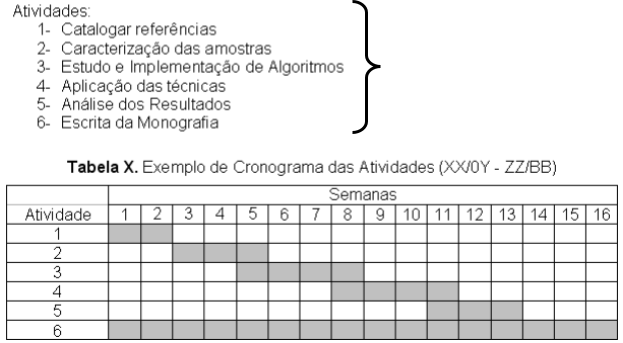
\includegraphics[width=0.9\textwidth]{images/cronograma_exemplo.png}
\end{figure}

% =========================================
% REFERÊNCIAS
% =========================================

\newpage
% Remove o título automático (limpa a macro que gera o nome)
\renewcommand{\bibname}{}

% Se o seu modelo usa a classe 'article', use este também por garantia:
\renewcommand{\refname}{}

\section{Referências Bibliográficas}

\vspace{-0.4cm}

\noindent\rule{\textwidth}{0.7pt}

<Coloque suas referencias no arquivo referencias.bib, quando elas forem citadas no texto iram aparecer aqui, como por exemplo \cite{silva2024} e \cite{knuth1984}>

\vspace{-0.8cm}

\bibliography{referencias}

\end{document}
